% --------
% --------
\section{Modelo DOT}

\begin{frame}{El Modelo DOT: Regeneración Urbana Sistémica}
    \begin{block}{Definición y Objetivo}
        El Desarrollo Orientado al Transporte (DOT) busca crear núcleos compactos de usos mixtos alrededor de estaciones 
        de transporte masivo para revertir la dependencia del automóvil.
    \end{block}

    \begin{columns}[T]
        \begin{column}{0.38\textwidth}
            \centering
            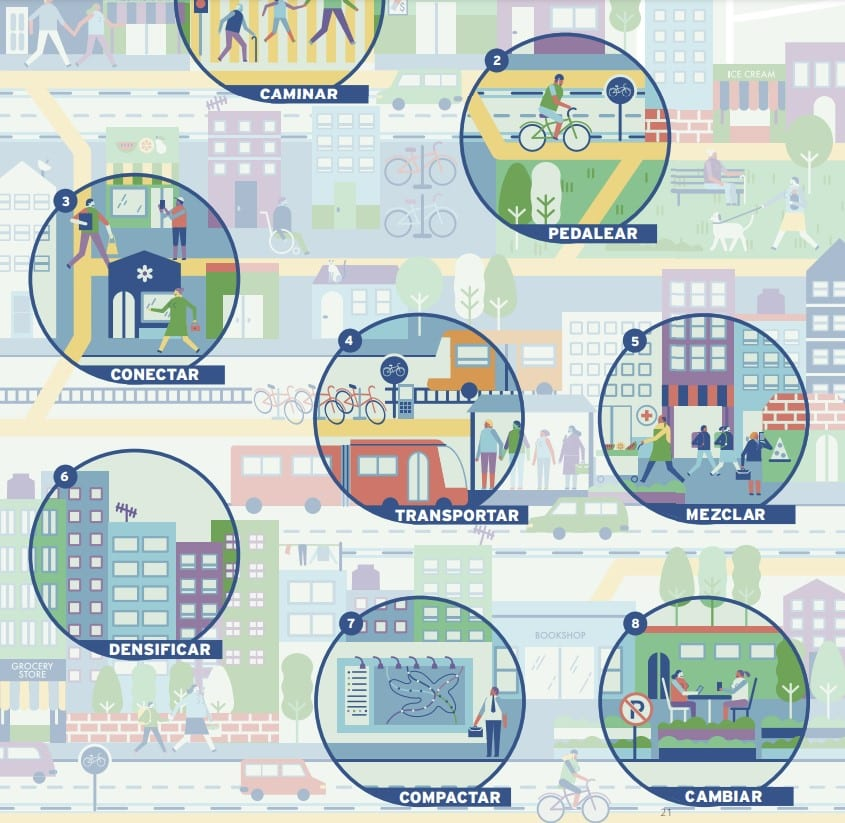
\includegraphics[width=\textwidth]{img/Principios_itdp.jpg}
            \fuentefigura{Iconografía de los 8 Principios \cite{ITDP_Espacio}.}
        \end{column}
        \begin{column}{0.65\textwidth}
            \small
            \begin{itemize}
                \item \textbf{Caminar/Pedalear:} La movilidad activa como base de la intermodalidad \cite{RedalycPeaton}.
                \item \textbf{Densificar/Compactar:} Concentrar la vivienda donde existe infraestructura masiva \cite{SEDATU2023}.
                \item \textbf{Cambiar:} Reducción activa del espacio dedicado al vehículo particular.
            \end{itemize}
        \end{column}
    \end{columns}
\end{frame}

% --------
% --------
\begin{frame}{Métricas de Evaluación: Estándar ITDP}
    \begin{block}{Sistema de Puntuación (Oro, Plata, Bronce)}
        El estándar permite pasar de descripciones cualitativas a evaluaciones rigurosas de la integración transporte-suelo \cite{ITDP_Espacio}.
    \end{block}

    \begin{itemize}
        \item \textbf{Vivienda Asequible:} Garantizar que la densificación no desplace a la población original.
        \item \textbf{Fachadas Activas:} Diseño urbano que fomenta la seguridad ciudadana y la vitalidad económica.
    \end{itemize}
\end{frame}

% --------
% --------
\begin{frame}{Métricas de Evaluación: Estándar ITDP 2}
        \begin{itemize}
        \item \textbf{Justicia Socioespacial:} La infraestructura debe servir como herramienta de equidad en el acceso a la ciudad \cite{SEDATU2023}.
    \end{itemize}
    \begin{exampleblock}{Dato Crítico}
                Solo los proyectos que logran alta conectividad y usos mixtos reducen efectivamente las externalidades 
                del 4\% del PIB \cite{IMCO2019Doc}.
    \end{exampleblock}
\end{frame}

% --------
% --------
% --- SECCIÓN 4: REPORTE 02 ---
\begin{frame}{R-2: Metodología del Nivel de Cobertura ($C$)}
    \begin{block}{Indicador de Equidad Espacial}
        El presente indicador evalúa la equidad espacial de la red de transporte masivo, midiendo la capacidad del sistema para servir como columna 
        vertebral de la justicia socioespacial \cite{Garibaldi2024_R02, SEDATU2023}.
        \begin{equation}
            C = \left( \frac{A_{cubierta}}{A_{total}} \right) \times 100
        \end{equation}
    \end{block}

    \begin{itemize}
        \item \textbf{Isócrono de Accesibilidad Peatonal:} Se establece un radio de caminata (\textit{buffer}) de \textbf{800 metros} 
                alrededor de cada estación.
        \item \textbf{Umbral Temporal:} Este radio equivale a un trayecto de entre \textbf{10 a 15 minutos caminando}, 
                alineándose con los principios de Caminar y Conectar del estándar DOT \cite{ITDP_Espacio}.
    \end{itemize}
\end{frame}

% --- Diapositiva: Escenario Base - Zonas de Exclusión ---
\begin{frame}{Escenario Base: Zonas de Exclusión al Transporte Masivo}
    \begin{exampleblock}{Hallazgo Estadístico}
        \footnotesize Las demarcaciones del 3er y 4to contorno presentan un rezago crítico que invalida el principio de accesibilidad universal \cite{Garibaldi2024_R02, SEDATU2023}.
    \end{exampleblock}
    \begin{columns}[T]
        \begin{column}{0.90\textwidth}
            \centering
            \renewcommand{\arraystretch}{1.2} % Mejora el espacio entre filas
            \scriptsize
            \begin{table}[]
                \begin{tabular}{lccc}
                \hline
                \textbf{Demarcación} & \textbf{Área ($km^2$)} & \textbf{Cubierta} & \textbf{Cobertura} \\ \hline
                Milpa Alta           & 298.01                & 35.00             & \textbf{11.75\%}   \\
                Magdalena Contreras  & 63.37                 & 16.33             & \textbf{25.76\%}   \\
                Tlalpan              & 314.25                & 94.31             & \textbf{30.01\%}   \\
                Tláhuac              & 85.78                 & 43.85             & \textbf{51.12\%}   \\
                Cuajimalpa           & 71.10                 & 37.12             & \textbf{52.20\%}   \\ \hline
                \end{tabular}
                \caption{Peores 5 Coberturas - Alcaldías CDMX \cite{Garibaldi2024_R02}.}
            \end{table}
        \end{column}
    \end{columns}
\end{frame}

% --- Diapositiva: Mapa de Exclusión Espacial ---
\begin{frame}{Análisis de Exclusión Espacial: 4to Contorno}
    \begin{alertblock}{Exclusión Espacial}
        \scriptsize
        \begin{itemize}
            \item \textbf{Segregación:} El 4to contorno presenta la mayor brecha de acceso, marginando a las poblaciones periféricas de los servicios de transporte masivo \cite{Garibaldi2024_R02}.
            \item \textbf{Fallo del Modelo:} El diseño radial agota su capacidad operativa antes de alcanzar las zonas de conservación y la periferia popular \cite{Garibaldi2024VFT, Garibaldi2024_R02}.
        \end{itemize}
    \end{alertblock}
    \centering
    % Imagen del mapa en la parte superior para máximo impacto visual
    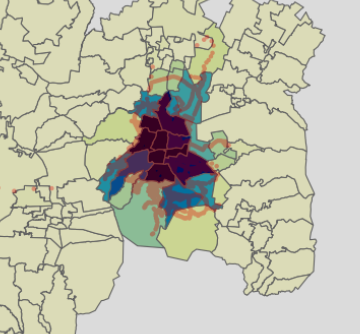
\includegraphics[width=0.85\textwidth, height=4.5cm, keepaspectratio]{img/cobertura_total_sistemas2.png}
    \fuentefigura{Elaboración propia: Análisis de Cobertura Capilar ($C$) \cite{Garibaldi2024_R02}.}
\end{frame}

% --- Diapositiva: Cobertura por Sistema (CC) ---
\begin{frame}{Cobertura por Sistema — Corredor Concesionado}
    \begin{block}{Concentración en el Núcleo Central}
        \begin{itemize}
            \scriptsize
            \item \textbf{Saturación Operativa:} La Cuauhtémoc y Benito Juárez presentan una malla de transporte redundante.
            \item \textbf{Contraste de Red:} Esta eficiencia central subraya la ineficiencia del modelo radial en las zonas periféricas analizadas previamente.
            \item \textbf{El sistema CC logra una cobertura casi total en el primer contorno, actuando como alimentador principal de la red masiva.}
        \end{itemize}
    \end{block}
    \begin{columns}[T]
        \begin{column}{0.60\textwidth}
            \centering
            \renewcommand{\arraystretch}{1.1}
            \scriptsize
            \begin{table}[]
                \begin{tabular}{lccc}
                \hline
                \textbf{Demarcación} & \textbf{Área ($km^2$)} & \textbf{Cubierta} & \textbf{Cobertura} \\ \hline
                Cuauhtémoc           & 32.50                 & 32.47             & \textbf{99.90\%}   \\
                Benito Juárez        & 26.68                 & 26.32             & \textbf{98.65\%}   \\
                Iztacalco            & 23.08                 & 22.25             & \textbf{96.42\%}   \\
                Miguel Hidalgo       & 46.39                 & 44.33             & \textbf{95.57\%}   \\
                Venustiano Carranza  & 33.84                 & 27.77             & \textbf{82.06\%}   \\ \hline
                \end{tabular}
            \end{table}
        \end{column}
        \begin{column}{0.38\textwidth}
            \centering
            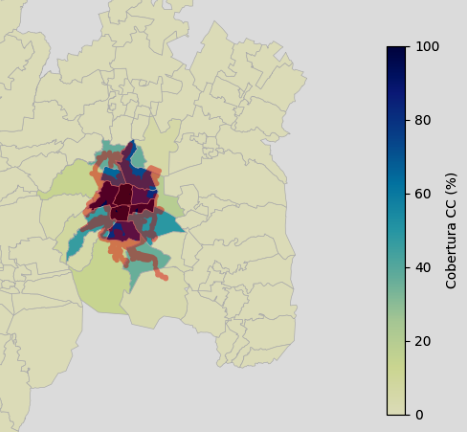
\includegraphics[width=\textwidth, height=4cm, keepaspectratio]{img/cobertura_cc.png}
            \fuentefigura{Análisis de Red Capilar \cite{Garibaldi2024_R02}.}
        \end{column}
    \end{columns}
\end{frame}

% --- Diapositiva: Cobertura por Sistema (RTP) ---
\begin{frame}{Cobertura por Sistema — RTP}
    \begin{block}{Distribución Estratégica y Conectividad Metropolitana}
        \begin{itemize}
            \scriptsize
            \item \textbf{Presencia en Demarcaciones Extensas:} A diferencia del modelo radial puro, el RTP mantiene coberturas superiores al 80\% en alcaldías críticas como Iztapalapa y Gustavo A. Madero \cite{Garibaldi2024_R02}.
            \item \textbf{Función Social y Equidad:} Actúa como el eje de movilidad de carácter social, extendiendo la red hacia zonas donde la topografía o la baja rentabilidad limitan al transporte concesionado \cite{Garibaldi2024_R02}.
            \item \textbf{Consolidación en Ejes Norte-Poniente:} Los niveles de cobertura cercanos al 90\% en Azcapotzalco y Miguel Hidalgo refuerzan la intermodalidad con los sistemas masivos del centro y periferia inmediata \cite{Garibaldi2024_R02}.
        \end{itemize}
    \end{block}
    \begin{columns}[T]
        \begin{column}{0.60\textwidth}
            \centering
            \renewcommand{\arraystretch}{1.1}
            \scriptsize
            \begin{table}[]
                \begin{tabular}{lccc}
                \hline
                \textbf{Demarcación} & \textbf{Área ($km^2$)} & \textbf{Cubierta} & \textbf{Cobertura} \\ \hline
                Miguel Hidalgo       & 46.39                 & 41.90             & \textbf{90.32\%}   \\
                Cuauhtémoc           & 32.50                 & 29.32             & \textbf{90.22\%}   \\
                Azcapotzalco         & 33.50                 & 30.08             & \textbf{89.81\%}   \\
                Gustavo A. Madero    & 87.84                 & 75.86             & \textbf{86.37\%}   \\
                Iztapalapa           & 113.07                & 93.66             & \textbf{82.83\%}   \\ \hline
                \end{tabular}
                \caption{Top 5 Alcaldías con mayor cobertura del Sistema RTP \cite{Garibaldi2024_R02}.}
            \end{table}
        \end{column}
        \begin{column}{0.38\textwidth}
            \centering
            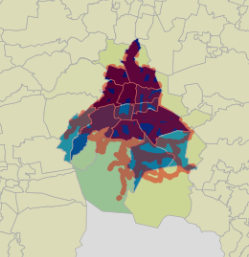
\includegraphics[width=\textwidth, height=4cm, keepaspectratio]{img/cobertura_rtp.png}
            \fuentefigura{Análisis de Red Capilar \cite{Garibaldi2024_R02}.}
        \end{column}
    \end{columns}
\end{frame}

% --- Diapositiva: Cobertura por Sistema (TROLE) ---
\begin{frame}{Cobertura por Sistema — Trolebús}
    \begin{block}{Ejes Eléctricos y Sustentabilidad Local}
        \begin{itemize}
            \scriptsize
            \item \textbf{Consolidación en el Eje Central-Sur:} Las alcaldías Cuauhtémoc (69.9\%) y Benito Juárez (61.8\%) 
                    lideran la cobertura, reflejando la infraestructura histórica de los corredores "Cero Emisiones".
            \item \textbf{Limitación de Penetración Capilar:} A diferencia del RTP, el Trolebús presenta coberturas más 
                    localizadas, funcionando como ejes troncales eléctricos en lugar de una red capilar extensiva.
            \item \textbf{Vínculo con la Ciudad Compacta:} Su alta eficiencia en Iztacalco y Coyoacán refuerza la 
                    viabilidad de modelos DOT en zonas con infraestructura eléctrica preexistente.
        \end{itemize}
    \end{block}
    \begin{columns}[T]
        \begin{column}{0.60\textwidth}
            \centering
            \renewcommand{\arraystretch}{1.1}
            \scriptsize
            \begin{table}[]
                \begin{tabular}{lccc}
                \hline
                \textbf{Demarcación} & \textbf{Área ($km^2$)} & \textbf{Cubierta} & \textbf{Cobertura} \\ \hline
                Cuauhtémoc           & 32.50                 & 22.72             & \textbf{69.90\%}   \\
                Benito Juárez        & 26.68                 & 16.50             & \textbf{61.85\%}   \\
                Azcapotzalco         & 33.50                 & 17.48             & \textbf{52.18\%}   \\
                Iztacalco            & 23.08                 & 11.93             & \textbf{51.69\%}   \\
                Coyoacán             & 53.88                 & 25.17             & \textbf{46.71\%}   \\ \hline
                \end{tabular}
            \end{table}
        \end{column}
        \begin{column}{0.38\textwidth}
            \centering
            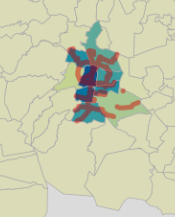
\includegraphics[width=\textwidth, height=4cm, keepaspectratio]{img/cobertura_trole.png}
            \fuentefigura{Análisis de Red Eléctrica \cite{Garibaldi2024_R02}.}
        \end{column}
    \end{columns}
\end{frame}

% --- Diapositiva: Cobertura por Sistema (MEXIBÚS) ---
\begin{frame}{Cobertura por Sistema — Mexibús}
    \begin{block}{Conectividad Metropolitana y Eficiencia Periférica}
        \begin{itemize}
            \scriptsize
            \item \textbf{Naturaleza Inter-metropolitana:} La cobertura es marginal dentro de la CDMX, ya que su función primordial 
                    es la alimentación masiva desde el Estado de México hacia los CETRAMs estratégicos.
            \item \textbf{Puntos de Interceptación Troncal:} Su presencia se limita a alcaldías colindantes como Iztacalco y 
                    Gustavo A. Madero, actuando como un sistema de "penetración" y no de cobertura capilar.
            \item \textbf{Integración Sistémica:} Los bajos porcentajes (máximo 6.58\%) demuestran que el sistema Mexibús requiere
                     de una infraestructura de interceptación anillar para distribuir eficientemente sus flujos en la periferia de la CDMX.
        \end{itemize}
    \end{block}
    \begin{columns}[T]
        \begin{column}{0.60\textwidth}
            \centering
            \renewcommand{\arraystretch}{1.1}
            \scriptsize
            \begin{table}[]
                \begin{tabular}{lccc}
                \hline
                \textbf{Demarcación} & \textbf{Área ($km^2$)} & \textbf{Cubierta} & \textbf{Cobertura} \\ \hline
                Iztacalco            & 23.08                 & 1.52              & \textbf{6.58\%}    \\
                Venustiano Carranza  & 33.84                 & 1.90              & \textbf{5.62\%}    \\
                Gustavo A. Madero    & 87.84                 & 3.23              & \textbf{3.67\%}    \\ \hline
                \end{tabular}
            \end{table}
        \end{column}
        \begin{column}{0.38\textwidth}
            \centering
            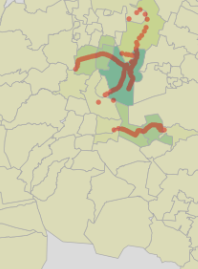
\includegraphics[width=\textwidth, height=4cm, keepaspectratio]{img/cobertura_mexibus.png}
            \fuentefigura{Análisis de Conectividad ZMVM \cite{Garibaldi2024_R02}.}
        \end{column}
    \end{columns}
\end{frame}

% --- Diapositiva: Cobertura por Sistema (MB) ---
\begin{frame}{Cobertura por Sistema — Metrobús}
    \begin{block}{Ejes Troncales de Alta Capacidad y Conectividad Central}
        \begin{itemize}
            \scriptsize
            \item \textbf{Eje de Alta Capacidad:} El Metrobús actúa como la columna vertebral de superficie, con una 
                    cobertura crítica en el corredor central, liderado por la Cuauhtémoc con un 82.27\%.
            \item \textbf{Consolidación en el Segundo Contorno:} Niveles superiores al 60\% en Benito Juárez e Iztacalco 
                    demuestran la madurez de los corredores BRT en la zona intermedia de la ciudad.
            \item \textbf{Eficiencia en la Intermodalidad:} Su rol es fundamental para la transferencia de usuarios hacia 
                    el Metro y la captación de viajes de la periferia, aunque su cobertura porcentual disminuye drásticamente 
                        en alcaldías de gran extensión territorial.
        \end{itemize}
    \end{block}
    \begin{columns}[T]
        \begin{column}{0.60\textwidth}
            \centering
            \renewcommand{\arraystretch}{1.1}
            \scriptsize
            \begin{table}[]
                \begin{tabular}{lccc}
                \hline
                \textbf{Demarcación} & \textbf{Área ($km^2$)} & \textbf{Cubierta} & \textbf{Cobertura} \\ \hline
                Cuauhtémoc           & 32.50                 & 26.74             & \textbf{82.27\%}   \\
                Benito Juárez        & 26.68                 & 16.21             & \textbf{60.74\%}   \\
                Iztacalco            & 23.08                 & 13.95             & \textbf{60.44\%}   \\
                Venustiano Carranza  & 33.84                 & 16.10             & \textbf{47.58\%}   \\
                Gustavo A. Madero    & 87.84                 & 38.75             & \textbf{44.12\%}   \\ \hline
                \end{tabular}
            \end{table}
        \end{column}
        \begin{column}{0.38\textwidth}
            \centering
            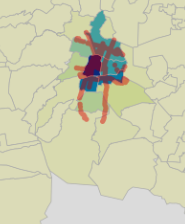
\includegraphics[width=\textwidth, height=4cm, keepaspectratio]{img/cobertura_mb.png}
        \end{column}
    \end{columns}
\end{frame}

% --- Diapositiva: Cobertura por Sistema (METRO) ---
\begin{frame}{Cobertura por Sistema — METRO}
    \begin{block}{La Columna Vertebral del Modelo Radial}
        \begin{itemize}
            \scriptsize
            \item \textbf{Predominancia en el Núcleo Central:} La Cuauhtémoc (87.23\%) y Benito Juárez (79.99\%) consolidan 
                al Metro como el eje estructural de alta capacidad, garantizando el derecho a la movilidad en el centro.
            \item \textbf{Saturación de Transferencia:} El sistema opera como el tronco principal de la "Higuera", donde el 
                diseño radial fuerza la convergencia de flujos hacia el centro, limitando las opciones de movilidad transversal.
            \item \textbf{Agotamiento en el Segundo Contorno:} Iztacalco y Azcapotzalco presentan coberturas moderadas ($\sim$50\%-41\%), 
                evidenciando que el Metro requiere de una red alimentadora robusta para servir a la periferia inmediata.
        \end{itemize}
    \end{block}
    \begin{columns}[T]
        \begin{column}{0.60\textwidth}
            \centering
            \renewcommand{\arraystretch}{1.1}
            \scriptsize
            \begin{table}[]
                \begin{tabular}{lccc}
                \hline
                \textbf{Demarcación} & \textbf{Área ($km^2$)} & \textbf{Cubierta} & \textbf{Cobertura} \\ \hline
                Cuauhtémoc           & 32.50                 & 28.35             & \textbf{87.23\%}   \\
                Benito Juárez        & 26.68                 & 21.34             & \textbf{79.99\%}   \\
                Venustiano Carranza  & 33.84                 & 24.39             & \textbf{72.07\%}   \\
                Iztacalco            & 23.08                 & 11.66             & \textbf{50.52\%}   \\
                Azcapotzalco         & 33.50                 & 13.80             & \textbf{41.19\%}   \\ \hline
                \end{tabular}
            \end{table}
        \end{column}
        \begin{column}{0.38\textwidth}
            \centering
            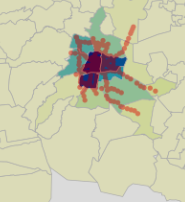
\includegraphics[width=\textwidth, height=4cm, keepaspectratio]{img/cobertura_metro.png}
            \fuentefigura{Análisis de Red Masiva Subterránea \cite{Garibaldi2024_R02}.}
        \end{column}
    \end{columns}
\end{frame}

% --- Diapositiva: Cobertura por Sistema (CB) ---
\begin{frame}{Cobertura por Sistema — Cablebús}
    \begin{block}{Justicia Social y Conectividad en Topografías Complejas}
        \begin{itemize}
            \scriptsize
            \item \textbf{Solución de Movilidad Periférica:} El Cablebús conecta zonas de difícil acceso en GAM e Iztapalapa, 
                logrando reducciones en los tiempos de traslado de hasta un 45\%.
            \item \textbf{Impacto Ambiental y Seguridad:} Ha permitido mitigar más de 18,000 toneladas de CO2 y se reporta 
                como uno de los sistemas más seguros debido a su monitoreo constante.
            \item \textbf{Baja Cobertura Espacial, Alta Eficiencia Local:} Aunque su cobertura ($C$) es menor al 13\%, 
                su relevancia radica en proveer accesibilidad capilar en territorios históricamente segregados.
        \end{itemize}
    \end{block}
    \begin{columns}[T]
        \begin{column}{0.60\textwidth}
            \centering
            \renewcommand{\arraystretch}{1.1}
            \scriptsize
            \begin{table}[]
                \begin{tabular}{lccc}
                \hline
                \textbf{Demarcación} & \textbf{Área ($km^2$)} & \textbf{Cubierta} & \textbf{Cobertura} \\ \hline
                Gustavo A. Madero    & 87.84                 & 11.31             & \textbf{12.88\%}   \\
                Miguel Hidalgo       & 46.39                 & 5.50              & \textbf{11.85\%}   \\
                Iztapalapa           & 113.07                & 12.74             & \textbf{11.27\%}   \\
                Álvaro Obregón       & 95.82                 & 4.38              & \textbf{4.57\%}    \\ \hline
                \end{tabular}
            \end{table}
        \end{column}
        \begin{column}{0.38\textwidth}
            \centering
            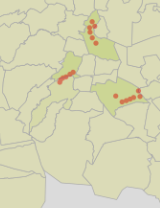
\includegraphics[width=\textwidth, height=4cm, keepaspectratio]{img/cobertura_cbb.png}
        \end{column}
    \end{columns}
\end{frame}